\section{LOS Coverage Map}\label{sec:los_map}
A point of interest of the project is to know if there is Line-Of-Sight (LOS) between the groundstation (GNS) and the drone. This has been done on a topographic map which takes into account:

\begin{itemize}
	\item Terrain elevation
	\item Curvature of the Earth
	\item Height of receiver and transmitter
\end{itemize}

In this sense, a MATLAB script has been addressed which at first imports a Web Map Service (WMS) to load the topographic map. The map captures the terrain in Denmark and some of its surroundings as seen in Figure \ref{fig:dk_map}.

\begin{figure}[h]
	\centering
	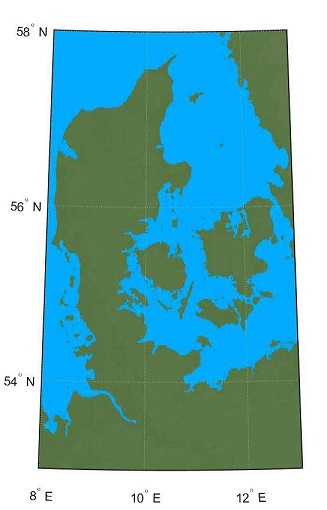
\includegraphics[scale=2]{figures/denmark.jpg}
	\caption{Topographic map of Denmark}
   	\label{fig:dk_map}
\end{figure}

Given the map and the topographic data in Figure \ref{fig:dk_map}, now it is possible to input the desired points for the GNS and the drone. As mentioned above, there are some parameters taken into account for plotting the LOS distance between the two points of interest. This distance can be seen in Figure \ref{fig:los_2p}, where the LOS is lost after 50 kilometers from the GNS.

\begin{figure}[h]
	\centering
	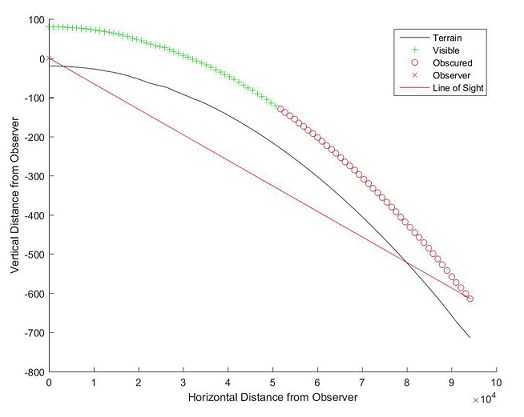
\includegraphics[scale=2.5]{figures/los_2points.jpg}
	\caption{LOS between GNS and drone \\ X axis - LOS distance [m] \\ Y axis - Altitude [m]}
   	\label{fig:los_2p}
\end{figure}

Moving further, for the same map (Figure \ref{fig:dk_map}) a location for the GNS can be chosen, such that it will result into a LOS area (white zone) as seen in Figure \ref{fig:los_area}. This area is also referred as the LOS coverage map.

\begin{figure}[h]
	\centering
	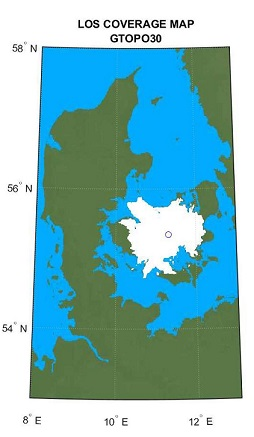
\includegraphics[scale=2.5]{figures/coverage_map.jpg}
	\caption{LOS Coverage Map from the GNS}
   	\label{fig:los_area}
\end{figure}

It can be observed from Figure \ref{fig:los_area} that in some areas of the map there is no visibility, due to higher terrain elevation. This can be overcome by increasing the GNS and/or drone altitude, such that we achieve LOS.  

Taking into account that a MATLAB script has been achieved, a thourough working principle has to be addressed in the following steps:
\begin{itemize}
	\item Aquire topography map 
	\item Input GNS and drone altitudes
	\item Choose locations for GNS and drone on (click) the map in order to plot LOS distance
	\item Choose (click) location of the GNS in order to plot LOS coverage map
\end{itemize}